\documentclass[a4paper, 10pt]{article}

% import packages
\usepackage[margin=0.2cm]{geometry}
\usepackage{pdflscape}
\usepackage{array}
\usepackage{makecell}
\usepackage{xcolor}
\usepackage{colortbl}
\usepackage{longtable}
\usepackage{titlesec}
\usepackage{float}
\usepackage{needspace}
\usepackage{graphicx}
\usepackage{hyperref}
\usepackage{setspace}
\usepackage{fancyhdr}
\usepackage{enumitem}
\usepackage{multicol}
\usepackage{amsmath}
\usepackage{graphicx}
\usepackage[table]{xcolor}
\usepackage{booktabs}   % for \toprule, \midrule, \bottomrule
\usepackage{adjustbox}  % for \begin{adjustbox}{max width=\textwidth}
\usepackage{etoolbox}
\usepackage{tikz}
\usepackage{caption}
\usetikzlibrary{arrows.meta, positioning, shapes.geometric,fit,calc}
\usepackage{pgfplots}
\usepgfplotslibrary{groupplots}
\pgfplotsset{compat=1.18}

% ---------- custom plot styles ----------
\pgfplotsset{
  acfstyle/.style={
    ycomb,
    mark=o,
    mark size=1.0pt, % <-- smaller circles
    mark options={solid, fill=white}
  }
}


\AtBeginEnvironment{tabular}{\tiny}
\definecolor{cDark}{HTML}{203F4A}
\definecolor{cTeal}{HTML}{1D8F7E}
\definecolor{cGold}{HTML}{E9C06A}
\definecolor{cOrange}{HTML}{F29B5C}
\definecolor{cRed}{HTML}{E85D47}

\renewcommand{\familydefault}{\sfdefault}

\newlength\tindent
\setlength{\tindent}{\parindent}
\setlength{\parindent}{0pt}
\renewcommand{\indent}{\hspace*{\tindent}}

% global list spacing (affects all levels)
\setlist{noitemsep, topsep=0pt, parsep=0pt, partopsep=0pt}

% now explicitly override indentation for each level you care about:
\setlist[itemize,1]{leftmargin=1.2em,label=\raisebox{0.5ex}{\scalebox{0.6}{$\bullet$}}}
\setlist[itemize,2]{leftmargin=1.4em}
\setlist[itemize,3]{leftmargin=0.5em}


\setlist[enumerate,1]{leftmargin=1.2em}
\setlist[enumerate,2]{leftmargin=1.4em}
\setlist[enumerate,3]{leftmargin=0.5em}

\setlength{\columnseprule}{0.1pt}
% ------------------------------------------------------


% Configure makecell package
\renewcommand{\theadalign}{bc}
\renewcommand{\theadgape}{\Gape[4pt]}
\renewcommand{\cellgape}{\Gape[4pt]}
\renewcommand{\cellalign}{lt}

% global line spacing
\renewcommand{\baselinestretch}{1.2}

% colour definitions
\definecolor{lightergray}{gray}{0.90}

\providecommand{\tightlist}{%
\setlength{\itemsep}{0pt}
\setlength{\parskip}{0pt}}

\begin{document}
  \begin{landscape}
\begin{multicols}{5}
\tiny

{\textbf{Statistische Charakter Zeitreihe:}}
Erwartungswert, Varianz, Trend, Saisonalität, korrelationsstruktur (ACF, PACF, CCF, ARIMA)

{\footnotesize{Analyse Prozess}}
\begin{enumerate}
    \item 1. Exploration \& Vorbereitung
    \begin{itemize}
        \item Zeitreihe Input \(\rightarrow\) Technische Vorbereitung
        \item Diskrete Zeit und Kontinuierlicher Wert
        \item Erkennen der grundstruktur, erfüllung technischer Anforderungen, keine lücken, vergleichen mit erwartungen, ergänzung wenn erforderlich
    \end{itemize}
    \item Modellierung: Zerlegung (Trend, Saisonalität, Residuen)
    \item Analyse von Residuen (Korrelation, Kreuzkorrelation / (partielle) autokorrelation)
    \item Stochastische Modellierung
    \begin{itemize}
        \item Trend / Saisonalität \(\rightarrow\) Vorhersage Erwartung
        \item Trend / Saisonalität \(\rightarrow\) Vorhersage seltene ereignisse
        \item Korrelationsanalysen \(\rightarrow\) Stochastische Modellierung \(\rightarrow\) Extremwert analyse
        \item Korrelationen / Stochastische Modellierung \(\rightarrow\) Einsicht (Zusammenhänge)
    \end{itemize}
\end{enumerate}


\vspace{0.4em}
\hrule
\vspace{0.7em}


{\scriptsize{2. Modellierung: Zerlegung}}

\begin{itemize}
    \item Trend (Glatte Komponente) (deterministisch): a long-term increasing or decreasing tendency
    \item Saisonalität (Periodische Komponente) (deterministisch): short-term repeating pattern at fixed periods, e.g., weekly, monthly
    \item Residuen (Stoachistische Komponente) \(\rightarrow\) Stationaritätstest
    \item Getan mit libraries und oder vorwissen
\end{itemize}

{\textbf{Zerlegung Zeitreihe \(x_n\)}}
\begin{itemize}    
    \item[1] Trend der unterschiede: kompromiss zwischen glattheit und info
    \item[2] Saisonal: rausnehmen, das überbleibsel ist sehr regelmässig
    \item[3] Residuen: Zeitreihe - Modell, sollten Normalverteilt sein, nicht über die Zeit korrelieren
    \item 3 komponenten Trend \(t_n\) , Saisonalität \(s_n\), error (residuen) \(\epsilon_n\)
    \item Additive decomposition \(x_n = t_n + s_n + \epsilon_n\) (multiplicative ersetzen mit multiplikation)
    \item Klassische Dekomposition: Moving Average
    \item LOESS Dekomposition: kontrolle über rolling window und period (moderner) (weight points in moving window that are closer stronger)
    \item Vorteile: Erklärungskraft der bekannten Vorgänge, stationäre residuen
\end{itemize}

{\textbf{Differenzierung}} ???

{\textbf{Stationarität}}
\begin{itemize}
    \item the concept that how a time series is changing will remain the same in the future 
    \item[1] Durchschnitt (konstant): ich habe alle änderungen im trend drinn, an den residuen ändert sich nichts mehr. Wenn jetzt der Durchschnitt ändert, dann folgt jetzt einer anderen regel wie in der vergangenheit \\ Ist ein Trend vorhanden?
    \item[2] Varianz (konstant): streuung muss konstant sein. Co-Varianz: zeitreihe zeitpunk T, verschiebung 4 lags, neuer Zeitpunkt verlgiech mit neuen lags. Wenn der zusammenhang besteht ist die varianz gleich \\ Ändert die Variabilität startk?
    \item[3] Saisonalität (keine): Ähnliche verteilung über der Zeit \\ Gibt es Regimewechsel?
    \item Es ändert sich nichts, voraussetzung für stochastische modellierung
    \item All white noise time series are stationary (similar conditions)
    \item (Augmented)-Dickey Fuller Test
    \begin{itemize}
        \item Is a type of test "Unit Root" is a characteristics that means that a time series is not stationary
        \item \(H_0\): \(lag_1 = 1\) that is the root of the augoregressiva lag (coefficient between lag 1) (non-stationary)
        \item \(H_1\): \(lag_1 < 1\) no unit root, it is stationary
    \end{itemize}
\end{itemize}


\vspace{0.4em}
\hrule
\vspace{0.7em}


{\scriptsize{3. Analyse}}


{\textbf{Autocorrelation Function (ACF)}}
\begin{itemize}
    \item 2 pieces both together
    \item \(S_{t-2} \rightarrow S_t\) direct route
    \item \(S_{t-2} \rightarrow S_{t-1} \rightarrow S_t\) indirect route
\end{itemize}

{\textbf{Partial Autocorrelation Function (PACF)}}
\begin{itemize}
    \item Coeefficient of S x lag ago on S today
    \item \(S_{t-2} \rightarrow S_t\) direct route 
    \item tells us if there is a direct effect from \(S_t\) to \(S_{t-2}\)
\end{itemize}

\vspace{0.4em}
\hrule
\vspace{0.7em}


{\scriptsize{4. Stochastische Modellierung}}


{\textbf{Autoregressive (AR) Modell}}
\begin{itemize}
    \item regression type: predict something based on the past values of that something
    \item 
\end{itemize}

{\textbf{MA-Modell}}
\begin{itemize}
    \item 
\end{itemize}


{\textbf{ARIMA}}
\begin{itemize}
    \item 
\end{itemize}


\vspace{0.4em}
\hrule
\vspace{0.7em}

    


\begin{itemize}
    \item {\textbf{Regelmässige Abtastung}} einteilung kontinuierliche Daten in Punkte (diskrete Zeit)
    \item {\textbf{Lag}} Zeitspanne vom einen zeitpunkt zum nächsten
    \item {\textbf{Extrapolation}} neue Daten ausserhalb der Zeitreihe, darf nicht machen, weil würde Modell auf sich selbst anwenden
    \item {\textbf{Interpolation / Imputation}} füllen Lücken innerhalb der Daten. Lineare Interpolation: Mit dem mittelwert zwischen zwei Zeitpunkten ergänzen. Forward / Backward Fill: jetztiger Zeitpunkt und fülle alle damit bis zum nächsten (ist schlechter). Kallman-Filter: guter filter für lange lückenmit viel struktur
    \item {\textbf{LOESS}} Seasonal Trend Decompose (STL), Multi- STL (MSTL)
    \item {\textbf{Parsimonous Model}} model kommt mit weniger parameter (bevorzugen) gleich gut wie mit mehr
    \item {\textbf{Kovarianten}} Die x externe faktoren
    \item {\textbf{Scheinkorrelation}} sieht korreliert aus hat aber nichts damit zu tun
    \item {\textbf{Granger kausalität}} Leading indicator, zeigt in die zukunft für die trailing variabel
    \item {\textbf{}}
    \item {\textbf{}}
    \item {\textbf{}}
\end{itemize}

\vspace{0.4em}
\hrule
\vspace{0.7em}


\end{multicols}

\tiny

{\footnotesize{Autokorrelation}}

\begin{itemize}
    \item (1) Periodisch, [2] white noise, [3] unklar ob absteigender trend, [4] kurzlebige zusammenhänge ist nicht noise
    \item[a] steigend \(\rightarrow\) 3
    \item[b] periodisch glatt schankend \(\rightarrow\) 1
    \item[c] sinkend \(\rightarrow\) 3
    \item[d] chaotisch \(\rightarrow\) 2 keine korrelation \& 4 gibt es noch zusammenhänge?
\end{itemize}


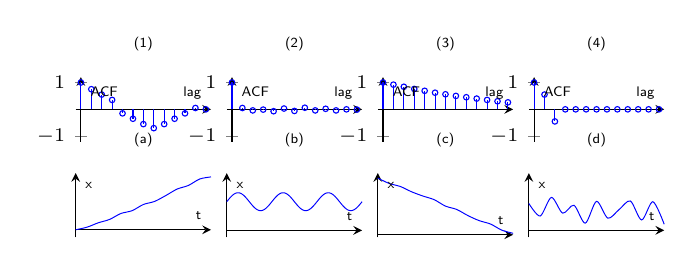
\begin{tikzpicture}
\begin{groupplot}[
  group style={
    group size=4 by 2,
    horizontal sep=0.2cm,
    vertical sep=0.4cm
  },
  width=3.3cm,
  height=2.4cm,
  axis lines=middle,
  xmin=-0.5, xmax=12.5,
  ymin=-1.2, ymax=1.2,
  xtick=\empty,
  ytick={-1,0,1},
  tick label style={font=\scriptsize},
  label style={font=\scriptsize},
  title style={font=\scriptsize},
  clip=false,
]

% ---------------- TOP ROW: ACF ----------------

% (1) alternating and dying out
\nextgroupplot[title={\tiny(1)}, xlabel={\tiny{lag}}, ylabel={\tiny{ACF}}]
\addplot+[acfstyle] coordinates {
 (0,1)
 (1,0.75) (2,0.55) (3,0.35)
 (4,-0.15) (5,-0.35) (6,-0.55) (7,-0.70)
 (8,-0.55) (9,-0.35) (10,-0.15) (11,0.05)
 (12,0)
};

% (2) only lag 0 spike
\nextgroupplot[title={\tiny(2)}, xlabel={\tiny{lag}}, ylabel={\tiny{ACF}}]
\addplot+[acfstyle] coordinates {
 (0,1)
 (1, 0.05) (2,-0.04) (3, -0.01) (4,-0.07) (5, 0.03) (6,-0.06)
 (7, 0.06) (8,-0.04) (9, 0.02) (10,-0.04) (11, 0.0) (12,-0.01)
};

% (3) positive decaying ACF
\nextgroupplot[title={\tiny(3)}, xlabel={\tiny{lag}}, ylabel={\tiny{ACF}}]
\addplot+[acfstyle] coordinates {
 (0,1)
 (1,0.92) (2,0.84) (3,0.76) (4,0.69) (5,0.62)
 (6,0.56) (7,0.50) (8,0.45) (9,0.40) (10,0.35)
 (11,0.30) (12,0.26)
};

% (4) two spikes then ~0
\nextgroupplot[title={\tiny(4)}, xlabel={\tiny{lag}}, ylabel={\tiny{ACF}}]
\addplot+[acfstyle] coordinates {
 (0,1)
 (1,0.55)
 (2,-0.45)
 (3,0) (4,0) (5,0) (6,0) (7,0)
 (8,0) (9,0) (10,0) (11,0) (12,0)
};

% ---------------- BOTTOM ROW: TIME SERIES ----------------

% (a) upward trend with small noise
\nextgroupplot[
  title={\tiny(a)},
  xmin=0, xmax=12,
  ymin=-0.3, ymax=2.2,
  xlabel={\tiny{t}}, ylabel={\tiny{x}},
  ytick=\empty
]
\addplot+[smooth, mark=none,line width=0.35pt] coordinates {
 (0,0.0) (1,0.10) (2,0.27) (3,0.40) (4,0.63) (5,0.74)
 (6,0.98) (7,1.10) (8,1.33) (9,1.58) (10,1.72) (11,1.97) (12,2.05)
};

% (b) oscillation
\nextgroupplot[
  title={\tiny(b)},
  xmin=0, xmax=12,
  ymin=-0.2, ymax=1.6,
  xlabel={\tiny{t}}, ylabel={\tiny{x}},
  ytick=\empty
]
\addplot+[smooth, mark=none,line width=0.35pt, samples=200, domain=0:12]
  {0.8 + 0.25*sin(deg(2*pi*x/4))};

% (c) downward trend with noise
\nextgroupplot[
  title={\tiny(c)},
  xmin=0, xmax=12,
  ymin=-0.1, ymax=2.2,
  xlabel={\tiny{t}}, ylabel={\tiny{x}},
  ytick=\empty
]
\addplot+[smooth, mark=none,line width=0.35pt] coordinates {
 (0,2.02) (1,1.83) (2,1.72) (3,1.53) (4,1.38) (5,1.25)
 (6,1.02) (7,0.90) (8,0.68) (9,0.50) (10,0.38) (11,0.16) (12,0.05)
};

% (d) stationary noise around constant level
\nextgroupplot[
  title={\tiny(d)},
  xmin=0, xmax=12,
  ymin=-0.2, ymax=1.6,
  xlabel={\tiny{t}}, ylabel={\tiny{x}},
  ytick=\empty
]
\addplot+[smooth, mark=none, line width=0.35pt] coordinates {
 (0,0.75) (1,0.40) (2,0.92) (3,0.48) (4,0.70) (5,0.2)
 (6,0.81) (7,0.34) (8,0.58) (9,0.82) (10,0.29) (11,0.80) (12,0.17)
};

\end{groupplot}
\end{tikzpicture}

\end{landscape}
\end{document}
